% math.tex — \input'd from thesis/experiments.tex
%
% Tests whether near-Lagrangian 2-faces (small |ω₀| between adjacent facets)
% act as obstacles that help create high systolic ratios.
%
% Sources:
%   - Generated data: experiments/omega-obstacle/omega-obstacle.jsonl
%   - Plot script: experiments/omega-obstacle/analyze.py
%   - Experiment notes: experiments/omega-obstacle/logbook.md
%
% Structure:
%   - Hypothesis and mechanism
%   - Phase A: observational (scatter plots, orbit vs non-orbit ω)
%   - Phase B: gradient analysis (⟨∂sys/∂a_k, ∂ω/∂a_k⟩ dot products)
%   - Known polytopes
%   - Conclusion

\subsection{Near-Lagrangian 2-Faces and Systolic Ratio}
\label{sec:omega-obstacle}

The HK-O counterexample is a perturbed Lagrangian product whose
optimal orbit traverses several ridges with $\omega_0(a_i, a_j) = 0$
(Lagrangian ridges).
This motivates the hypothesis that near-Lagrangian ridges --- facet
pairs with small $|\omega_0(a_i, a_j)|$ --- act as ``obstacles'' that
help create high systolic ratios.

\subsubsection*{Mechanism}

The connection between $\omega_0$ values and $\mathrm{sys}$ runs through
the quadratic form $Q(\beta)$ from Lemma~\ref{lem:H-quadratic}:
\[
  Q(\beta)
  = \sum_{j < i} \beta_i\,\beta_j\;\omega_0(a_{\sigma(j)},\, a_{\sigma(i)}).
\]
The capacity is $c_{\mathrm{EHZ}} = 1/(2\,Q^*)$, where $Q^*$ is the
maximum of~$Q$ subject to the KKT constraints.
If the $\omega_0$ values appearing in the sum are small, $Q^*$ could be
smaller, giving a larger capacity and potentially a larger
$\mathrm{sys} = c_{\mathrm{EHZ}}^2 / (2\,\mathrm{vol})$.

We test this hypothesis from two angles: an observational study
(Phase~A) correlating $\omega_0$ features with $\mathrm{sys}$ across a
large dataset, and a gradient analysis (Phase~B) asking whether the
$\mathrm{sys}$-increasing direction tends to decrease~$\omega_0$.

\subsubsection*{Dataset}

We generate 950 random polytopes: 200 each for $F \in \{5,6,7,8\}$,
100 for $F = 9$, and 50 for $F = 10$.
Facet normals are uniform on $S^3$, heights uniform in $[0.8, 1.2]$,
seed~42.
We add three known polytopes as reference points: the HK-O
counterexample ($\mathrm{sys} \approx 1.047$, $F = 10$), the simplex
($\mathrm{sys} = 0.75$, $F = 5$), and the hypercube
($\mathrm{sys} = 0.5$, $F = 8$).
Total: 953 polytopes.

For each polytope, we compute $c_{\mathrm{EHZ}}$ using the instrumented
HK2017 algorithm (which returns the optimal $\beta^*$, $\lambda$, $\nu$,
$Q^*$ from the KKT solve), the geometric skeleton (ridge adjacency via
shared 2-faces), and $\omega_0(a_i, a_j)$ for every ridge pair.

\subsubsection*{Phase A: Observational Correlations}

\paragraph{Ridge $\min|\omega_0|$ vs sys.}

Figure~\ref{fig:omega-ridge-min} plots, for each polytope, the
smallest $|\omega_0(a_i, a_j)|$ over all ridge pairs $(i,j)$
against~$\mathrm{sys}$.
The Spearman rank correlation is $\rho = -0.22$, $p = 8 \times 10^{-12}$:
polytopes with a smaller global $\min|\omega_0|$ tend to have slightly
higher~$\mathrm{sys}$.
However, the scatter is very wide, and the correlation is likely
confounded by facet count: more facets produce more ridge pairs and thus
more chances for a small $|\omega_0|$ by chance, while facet count itself
correlates positively with $\mathrm{sys}$ ($\rho = +0.37$).

\begin{figure}[ht]
\centering
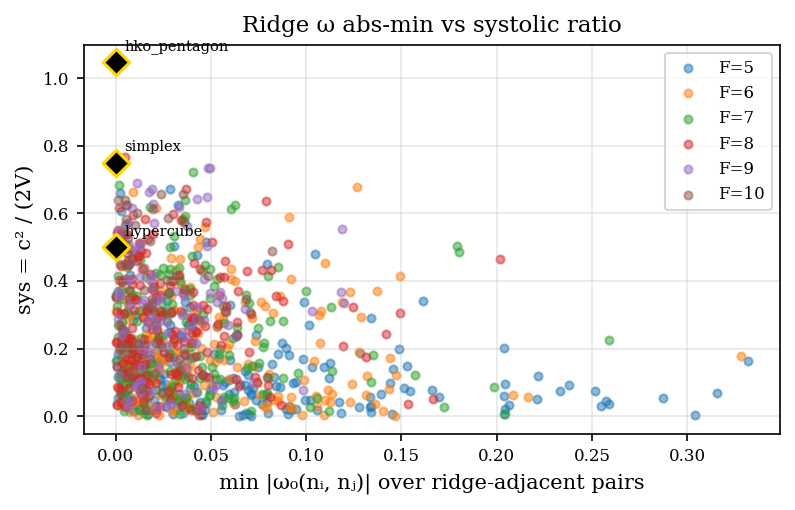
\includegraphics[width=0.9\textwidth]{../experiments/omega-obstacle/omega_obstacle_ridge_min_vs_sys.png}
\caption{Ridge $\min|\omega_0|$ vs.\ systolic ratio.
  Each point is one polytope, colored by facet count.
  Diamonds mark the three known polytopes.
  Spearman $\rho = -0.22$: weak negative correlation, likely confounded
  by facet count.}
\label{fig:omega-ridge-min}
\end{figure}

\paragraph{Orbit-specific $\omega_0$ features.}

The more focused test restricts to $\omega_0$ values along the
optimal orbit's consecutive facet transitions.
Neither the orbit minimum $\min_k |\omega_0(a_{\sigma(k)}, a_{\sigma(k+1)})|$
nor the orbit mean show any correlation with $\mathrm{sys}$:

\begin{center}
\begin{tabular}{lrr}
\toprule
Feature & Spearman $\rho$ & $p$-value \\
\midrule
orbit $\min|\omega_0|$ & $-0.02$ & $0.61$ \\
orbit mean $|\omega_0|$ & $+0.00$ & $0.99$ \\
\bottomrule
\end{tabular}
\end{center}

The $\omega_0$ values on the optimal orbit do not predict
$\mathrm{sys}$.

\paragraph{Orbit vs.\ non-orbit $|\omega_0|$ distribution.}

If the orbit were seeking small $\omega_0$ transitions, we would expect
orbit ridges to have systematically smaller $|\omega_0|$ than non-orbit
ridges.
The opposite is the case:
orbit ridges have median $|\omega_0| = 0.54$ (mean $0.52$), while
non-orbit ridges have median $|\omega_0| = 0.36$ (mean $0.40$).
The orbit preferentially uses facet transitions with \emph{large}
$|\omega_0|$.

This is consistent with the structure of the $Q$ maximization:
$Q(\beta) = \sum \beta_i \beta_j\,\omega_0(\ldots)$, so the optimizer
seeks large $\omega_0$ terms to maximize~$Q$.

\begin{figure}[ht]
\centering
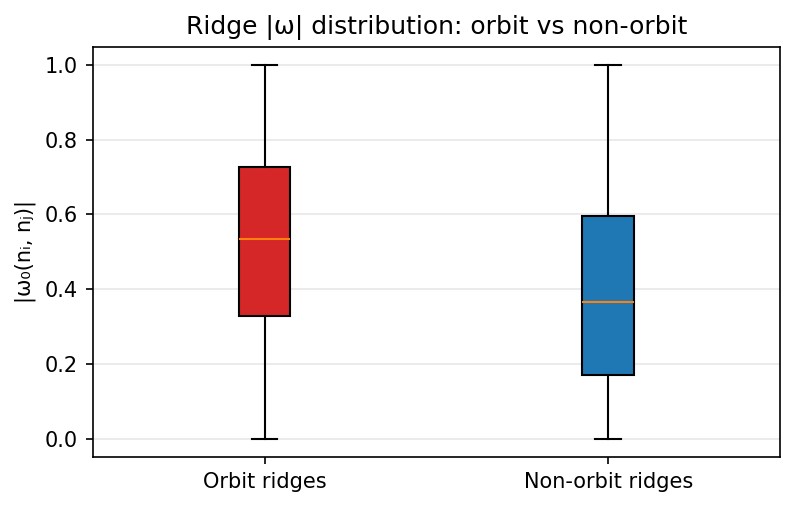
\includegraphics[width=0.7\textwidth]{../experiments/omega-obstacle/omega_obstacle_orbit_vs_nonorbit.png}
\caption{Distribution of $|\omega_0|$ for orbit ridges vs.\ non-orbit
  ridges across all 953 polytopes.
  The orbit preferentially uses transitions with large $|\omega_0|$,
  opposite to what the hypothesis predicts.}
\label{fig:omega-orbit-vs-nonorbit}
\end{figure}

\subsubsection*{Phase B: Gradient Analysis}

Phase~A shows no observational signal.
Phase~B asks the complementary question: does the
$\mathrm{sys}$-increasing direction in dual-vertex space tend to
\emph{decrease} $\omega_0$?

For each facet~$k$ and each ridge-neighbor~$i$, we compute:
\begin{enumerate}
\item $\frac{\partial\,\mathrm{sys}}{\partial a_k} \in \mathbb{R}^4$ ---
  the gradient of $\mathrm{sys}$ with respect to the dual vertex~$a_k$,
  using the analytical derivatives from
  Corollary~\ref{cor:sys-derivative} and
  Lemmas~\ref{lem:vol-derivative} and~\ref{lem:cap-derivative}:
  \[
    \frac{\partial\,\mathrm{sys}}{\partial a_k}
    = \frac{c_{\mathrm{EHZ}}}{\mathrm{vol}}\,
      \frac{\partial c_{\mathrm{EHZ}}}{\partial a_k}
    - \frac{c_{\mathrm{EHZ}}^2}{2\,\mathrm{vol}^2}\,
      \frac{\partial\,\mathrm{vol}}{\partial a_k}.
  \]
  For orbit facets, both volume and capacity contribute; for non-orbit
  facets, only the volume term is nonzero
  (since $\partial c_{\mathrm{EHZ}}/\partial a_k = 0$ when
  $k \notin S$).

\item $\frac{\partial}{\partial a_k}\omega_0(a_k, a_i) \in \mathbb{R}^4$ ---
  the gradient of $\omega_0(a_k, a_i)$ with respect to~$a_k$.
  Since $\omega_0(u, v) = u^T M\,v$ where $M = J_0^T = -J_0$,
  this is simply $-J_0\,a_i$.

\item The dot product
  $d = \bigl\langle \frac{\partial\,\mathrm{sys}}{\partial a_k},\;
        \frac{\partial}{\partial a_k}\omega_0(a_k, a_i) \bigr\rangle$.
\end{enumerate}

If $d < 0$ systematically, the $\mathrm{sys}$-increasing direction
also decreases $\omega_0$ --- supporting the hypothesis.
If $d$ is centered on zero, there is no directional relationship.

Figure~\ref{fig:omega-gradient} shows the distribution of~$d$
restricted to orbit facets (where the capacity gradient is nonzero).
The distribution is centered on zero:
median $d = +0.0006$, fraction negative $= 49.5\%$.
There is no evidence that the $\mathrm{sys}$-increasing direction
coincides with the $\omega_0$-decreasing direction.

\begin{figure}[ht]
\centering
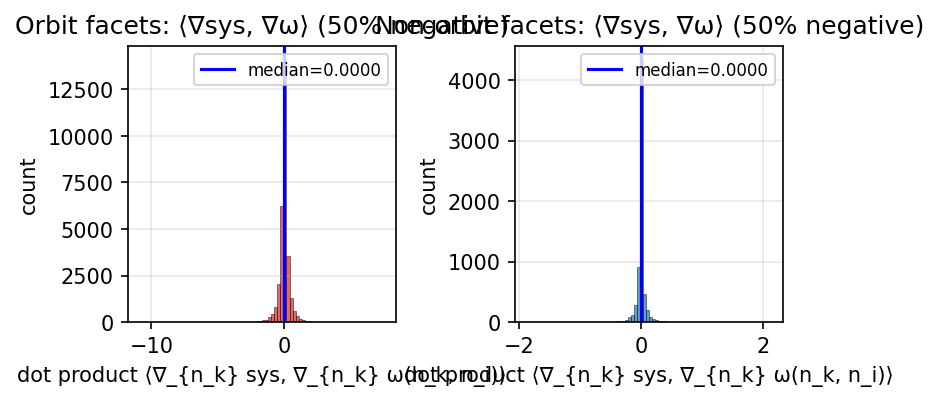
\includegraphics[width=0.9\textwidth]{../experiments/omega-obstacle/omega_obstacle_gradient_dots.png}
\caption{Distribution of $\bigl\langle \frac{\partial\,\mathrm{sys}}{\partial a_k},\,
  \frac{\partial}{\partial a_k}\omega_0(a_k, a_i) \bigr\rangle$ for orbit facets.
  The distribution is symmetric around zero --- no directional signal.}
\label{fig:omega-gradient}
\end{figure}

Figure~\ref{fig:omega-vs-dot} shows the dot product~$d$ against the
current $|\omega_0(a_k, a_i)|$.
The scatter exhibits a trumpet shape: variance increases at small
$|\omega_0|$, but the distribution remains centered on zero at all
$|\omega_0|$ values.
In particular, there is no special behavior near $|\omega_0| \approx 0$
(the near-Lagrangian regime).

\begin{figure}[ht]
\centering
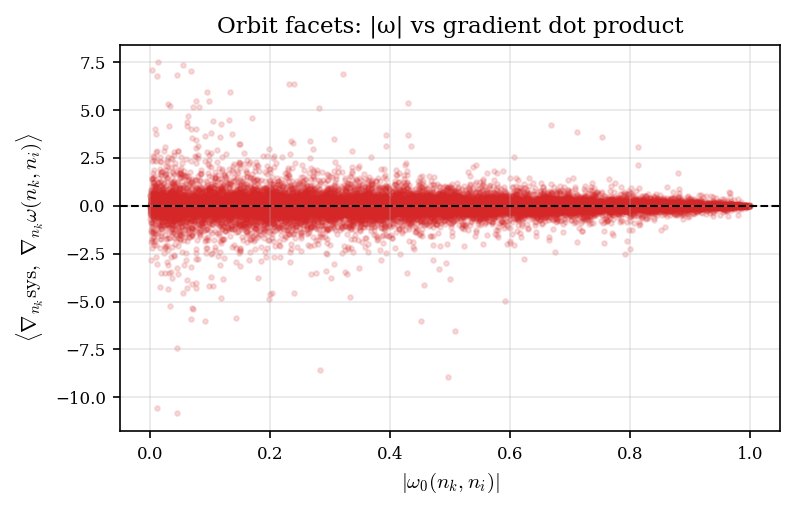
\includegraphics[width=0.9\textwidth]{../experiments/omega-obstacle/omega_obstacle_omega_vs_dot.png}
\caption{Dot product $\bigl\langle \frac{\partial\,\mathrm{sys}}{\partial a_k},\,
  \frac{\partial}{\partial a_k}\omega_0 \bigr\rangle$ vs.\ current $|\omega_0(a_k, a_i)|$
  for orbit facets.
  Trumpet shape: variance increases at small $|\omega_0|$, but the
  distribution is centered on zero throughout.}
\label{fig:omega-vs-dot}
\end{figure}

\subsubsection*{Known Polytopes}

\begin{center}
\small
\begin{tabular}{lrrrrl}
\toprule
Polytope & $F$ & sys & orbit $\min|\omega_0|$ &
  ridge $\min|\omega_0|$ & orbit len \\
\midrule
HK-O pentagon & 10 & 1.047 & 0.000 & 0.000 & 6 \\
Simplex       &  5 & 0.750 & 0.000 & 0.000 & 5 \\
Hypercube     &  8 & 0.500 & 1.000 & 0.000 & 4 \\
\bottomrule
\end{tabular}
\end{center}

All three have at least one Lagrangian ridge
($\mathrm{ridge}\;\min|\omega_0| = 0$), but the hypercube's optimal
orbit avoids Lagrangian ridges entirely
($\mathrm{orbit}\;\min|\omega_0| = 1.0$) yet has
$\mathrm{sys} = 0.5 < 1$.
The HK-O counterexample does have Lagrangian ridges on its orbit, but
this appears to be a consequence of its construction as a perturbed
Lagrangian product, not a general mechanism.

\subsubsection*{Conclusion}

The hypothesis that near-Lagrangian ridges help create high systolic
ratios is not supported by the data:
\begin{enumerate}
\item The weak global correlation ($\rho = -0.22$) between
  $\mathrm{ridge}\;\min|\omega_0|$ and $\mathrm{sys}$ is likely
  confounded by facet count.
\item Orbit-specific $\omega_0$ features show zero correlation with
  $\mathrm{sys}$.
\item The orbit preferentially uses \emph{large} $|\omega_0|$
  transitions, consistent with the $Q$-maximization structure.
\item The gradient analysis shows no directional relationship between
  $\partial\mathrm{sys}/\partial a_k$ and
  $\partial\omega_0/\partial a_k$.
\end{enumerate}

The mechanism linking small $\omega_0$ to large capacity --- while
mathematically valid ($Q$ has smaller terms $\to$ $Q^*$ could be
smaller) --- does not operate in practice because the KKT optimizer
compensates: it adjusts $\beta^*$ and selects orbits that maximize $Q$
despite small individual $\omega_0$ contributions.
